\section{Conception}

\subsection{Introduction}
\begin{prettyBox}{Conception Introduction}{mypur}
Conception represents the solution to a problem, expressed through structured diagrams such as UML.
Creating a conception is an iterative process that requires significant time and creativity.
Initially, a solution is developed, and subsequent iterations focus on optimizing it.

\vspace{0.15cm}
Each iteration refines and expands the conception until reaching a final result that is easy to
maintain. This ensures better implementation, facilitates adding or removing features, and 
simplifies bug fixes.

\end{prettyBox}

\vspace{0.5cm}
\begin{prettyBox}{Difference Between Conception \& UML}{red} 
    \begin{center} 
        \textbf{Conception $\not\Leftrightarrow$ UML} 
     \end{center}
UML is merely a tool used to represent the conception, it is not the conception itself. 
Conception encompasses more than just diagrams—it includes algorithms, explanations of 
diagrams, and other documents.
\end{prettyBox}


\vspace{0.5cm}
\begin{prettyBox}{Importance of Maintainability}{red} 
Easy maintainability is one of the key qualities of a good conception and arguably the most
important criteria. This is because we want the software to be long-lasting, and effective 
maintenance is essential to achieving that.
\end{prettyBox}

\vspace{0.5cm}
\subsection{Itterative Process Of Conception}

\begin{prettyBox}{Global \& Detailed Conception}{mypur}
    \begin{itemize}
        \item \textbf{Globale Conception :} Modules must be identified (some modules can 
be divided into sub-modules) , and interaction between modules must be defined
        \item \textbf{Detailed Conception :} Each module must be defined independently in detail.
    \end{itemize}
The conception should have high ratio of cohesion and low ratio of coupling
\end{prettyBox}

\vspace{0.5cm}

\begin{prettyBox}{Why Global Conception Then Detailed Conception}{red} 
    We first define the high-level structure of the modules and their interactions to provide an overall system architecture.
    This gives a clear overview of the software before delving into the detailed characteristics of each module.
\end{prettyBox}

\vspace{0.5cm}


\begin{prettyBox}{Why High Cohesion \& Low Coupling}{red}
    \begin{itemize}
        \item \textbf{Cohesion}: How related the responsibilities of a module are.
            \begin{itemize}
                \item \textbf{High Cohesion}: The module has a clear, well-defined responsibility, making it easier to understand, maintain, and modify.
                \item \textbf{Low Cohesion}: The module handles multiple, unrelated responsibilities, making it harder to maintain and understand.
            \end{itemize}
        \item \textbf{Coupling}: How dependent the modules are on each other.
            \begin{itemize}
                \item \textbf{High Coupling}: Modules are highly dependent on each other. A failure in one critical module may cause the entire system to fail.
                \item \textbf{Low Coupling}: Modules are loosely connected, and changes or failures in one module are less likely to impact the others.
            \end{itemize}
    \end{itemize}
    
    \textbf{Why We Want High Cohesion and Low Coupling}:
    \begin{itemize}
        \item \textbf{High Cohesion}: Ensures that each module has a clear, understandable purpose, making the system easier to maintain and extend.
        \item \textbf{Low Coupling}: Reduces dependencies between modules, minimizing the risk of widespread system failure and increasing flexibility.
    \end{itemize}
\end{prettyBox}


\vspace{0.5cm}

\subsection{Classification Of Conception Method}

\vspace{0.25cm}
\subsubsection{Function Oriented Conception}

\vspace{0.25cm}
\begin{prettyBox}{Function-Oriented}{mypur}
    The software is structured using a functional paradigm. It is divided into a set of functions 
that interact with each other. The software is viewed as a complex main function that is 
progressively decomposed into smaller, less complex sub-functions. This process continues until
we reach a detailed conception.

    \vspace{0.15cm}
    Each function has its own local state (local variables), while the software has
a global state (global variables) that is shared among all functions.
\end{prettyBox}

\vspace{0.5cm}
\subsubsection{Object Oriented Conception}

\vspace{0.25cm}

\begin{prettyBox}{Object-Oriented Design}{mypur}
    The software is viewed as a collection of encapsulated and independent objects. 
These objects communicate with each other by sending messages (method calls).

    \vspace{0.15cm}
    Each object is identified by its name and encapsulated attributes (variables and methods).
\end{prettyBox}


\vspace{0.5cm}

\subsubsection{Data Oriented Conception}

\vspace{0.25cm}

\begin{prettyBox}{Data-Oriented}{mypur}
    The software's structure must reflect the structure of the data it traits .
    Therefore the conception is influenced by the ouput input data.
\end{prettyBox}


\subsection*{\underline{Example :}}
Compiler

\vspace{1cm}

\subsection{Conception's Principales}To make sure the conception ensures an easily maintainable
software we must follow some printcipales :


\begin{prettyBox}{Principles}{mypur}

\begin{itemize}
    \item \textbf{Abstraction:} Focuses on the essential characteristics while
hiding unnecessary details.
    \item \textbf{Modularity:} Divides the system into modules with well-defined interactions,
adhering to the principle of high cohesion and low coupling.
    \item \textbf{Encapsulation:} Hides internal details of a module from other modules.
    \item \textbf{Structuring:} Ensures a structured conceptions (levels) , we can at least have general \& detailed conception.
\end{itemize}

\end{prettyBox}

\vspace{0.5cm}

\subsection{Notation For Fonctional Conception}


\begin{prettyBox}{Notation}{mypur}
\begin{itemize}
    \item \textbf{Data Flow Diagram (DFD):} Shows how data is transformed and passed from one module to another.
    \item \textbf{Structure Diagram (SD):} A hierarchical diagram that illustrates the structured relationships between the components of the software.
\end{itemize}
\end{prettyBox}


\vspace{0.5cm}

\begin{prettyBox}{Relation Between DFD \& SD}{red}
    DFD and SD are complementary to each other, working together to clearly describe the functional design of a software system.
\end{prettyBox}

\vspace{0.5cm}

\subsubsection{DFD}

\vspace{0.25cm}

\begin{prettyBox}{DFD}{mypur}
    A DFD diagram consists of four components:
    \begin{itemize}
        \item \textbf{Transformations}: Represented as circles.
        \item \textbf{Data}: Represented as axis.
        \item \textbf{Logical AND}: Represented by the symbol *.
        \item \textbf{Logical OR}: Represented by the symbol +.
    \end{itemize}
\end{prettyBox}

\vspace{0.5cm}

\begin{center}
    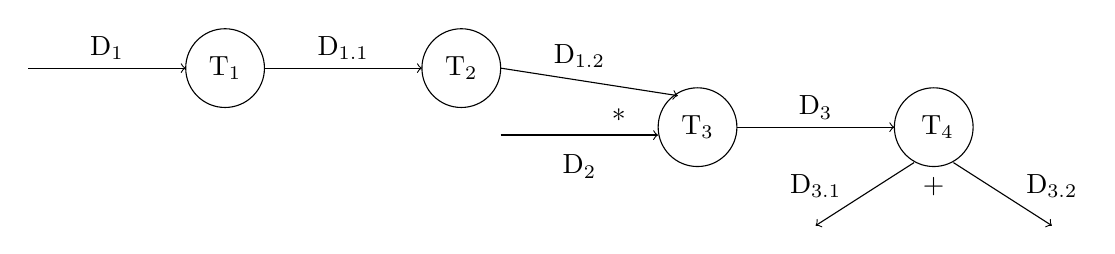
\begin{tikzpicture}
        \draw[->] (0,0) -- (2,0);
        \node at (1,0.25){D$_{1}$};
        \draw (2.5,0) circle (0.5);
        \node at (2.5,0) {T$_{1}$};
        
        \draw[->] (3,0) -- (5,0);
        \node at (4,0.25){D$_{1.1}$};
        \draw (5.5,0) circle (0.5);
        \node at (5.5,0) {T$_{2}$};

        \draw[->] (6,0) -- (8.25,-0.35);
        \node at (7,0.15){D$_{1.2}$};
        \draw (8.5,-0.75) circle (0.5);
        \node at (8.5,-0.75) {T$_{3}$};
        
        \draw[->] (6,-0.85) -- (8,-0.85);
        \draw[->] (9,-0.75) -- (11,-0.75);
        \node at (7.5,-0.65) {*};
        \node at (7,-1.25) {D$_{2}$};
        \node at (10,-0.5) {D$_{3}$};
        \draw (11.5,-0.75) circle (0.5);
        \node at (11.55,-0.75) {T$_{4}$};
        \draw[->] (11.25,-1.2) -- (10,-2);

        \node at (11.5,-1.5) {+};
        \draw[->] (11.75,-1.2) -- (13,-2);

        \node at (13,-1.5) {D$_{3.2}$};

        \node at (10,-1.5) {D$_{3.1}$};

    \end{tikzpicture}
\end{center}

\vspace{0.5cm}

\begin{prettyBox}{Note}{red}
    A DFD specifies the operations without detailing how they are performed. Each node in the diagram can be further described with another DFD, allowing for a hierarchical decomposition of processes.
\end{prettyBox}

\vspace{0.5cm}

\subsection*{\underline{Example :}}
